\subsection*{Singular Simplices}

\begin{definition}[Affinely Independent]
	Let $n,k \in \omega$. A family $(v_0,\dots,v_k)$ in $\mathbb{R}^n$ is said to be \bld{affinely independent}, iff the following condition is satisfied: Given $\lambda_0,\dots,\lambda_k \in \mathbb{R}$ such that
	\begin{equation*}
		\sum_{i = 0}^k \lambda_i = 0 \qquad \text{and} \qquad \sum_{i = 0}^k \lambda_i v_i = 0
	\end{equation*}
	\noindent implies $c_0 = \dots = c_k = 0$.
\end{definition}

\begin{lemma}
	\label{lem:affinely_independent}
	Let $n,k \in \omega$. Then a family $(v_0,\dots,v_k)$ in $\mathbb{R}^n$ is affinely independent if and only if $(v_1 - v_0,\dots,v_k - v_0)$ is linearly independent in $\mathbb{R}^n$.
\end{lemma}

\begin{exercise}
	\label{ex:affinely_independent}
	Prove lemma \ref{lem:affinely_independent}.
\end{exercise}

\begin{definition}[Simplex]
	\label{def:simplex}
	Let $n,k \in \omega$ and $(v_0,\dots,v_k)$ affinely independent in $\mathbb{R}^n$. Define the \bld{simplex spanned by $(v_0,\dots,v_k)$}, written $[v_0,\dots,v_k]$, to be the topological subspace 
	\begin{equation*}
		[v_0,\dots,v_k] := \cbr[4]{\sum_{i = 0}^k \lambda_i v_i : \lambda_i \in \mathbb{R}_{\geq 0} \> \text{and} \> \sum_{i = 0}^k \lambda_i = 1} \subseteq \mathbb{R}^n.
	\end{equation*}
	Moreover, each of the $v_i$'s, $i = 0,\dots,k$, is called a \bld{vertex} of the simplex $[v_0,\dots,v_k]$.
\end{definition}

\begin{remark}
	Let $\sigma := [v_0,\dots,v_k]$ be a simplex spanned by $(v_0,\dots,v_k)$. Then we will also simply call $\sigma$ a $k$-simplex in $\mathbb{R}^n$.
\end{remark}

\begin{example}[Standard Simplex]
	\label{ex:standard_simplex}
	Let $n \in \omega$. Then the family $(e_0,\dots,e_n)$ in $\mathbb{R}^n$, where $e_0 := 0$ and $(e_1,\dots,e_n)$ is the standard oriented basis of $\mathbb{R}^n$, is affinely independent by exercise \ref{ex:affinely_independent}. The $n$-simplex spanned by this family is called the \bld{standard $n$-simplex} and is denoted by $\Delta^n$.
	\begin{figure}[h!tb]
		\centering
		\begin{subfigure}[b]{.3\textwidth}
			\centering
			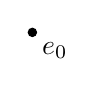
\begin{tikzpicture}[scale = 3]
				\draw[fill] (0,1) circle [radius=.5pt] node[below right]{$e_0$};
			\end{tikzpicture}
			\caption{$\Delta^0$.}
			\label{fig:Delta^0}
		\end{subfigure}
		~
		\begin{subfigure}[b]{.3\textwidth}
			\centering
			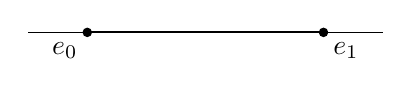
\begin{tikzpicture}[scale = 3]
    			% Draw axes
				\draw (-.75,1) -- (.75,1);
				\draw [thick] (-.5,1) -- (.5,1);
				\draw[fill] (-.5,1) circle [radius=.5pt] node[below left]{$e_0$};
				\draw[fill] (.5,1) circle [radius=.5pt] node[below right]{$e_1$};
			\end{tikzpicture}
			\caption{$\Delta^1$.}
			\label{fig:Delta^1}
		\end{subfigure}
		~
		\begin{subfigure}[b]{.3\textwidth}
			\centering
			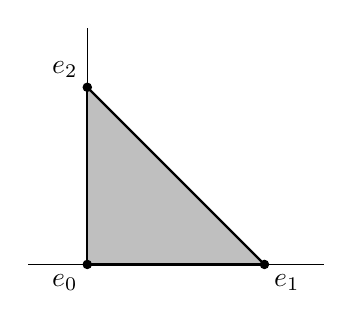
\begin{tikzpicture}[scale = 3]
    			% Draw axes
				\draw (-.25,1) -- (1,1);
				\draw (0,1) -- (0,2);
				\fill[fill=gray!50] (0,1)--(.75,1)--(0,1.75);
				\draw [thick] (0,1) -- (.75,1);
				\draw [thick] (0,1) -- (0,1.75);
				\draw [thick] (.75,1) -- (0,1.75);
				\draw[fill] (0,1) circle [radius=.5pt] node[below left]{$e_0$};
				\draw[fill] (.75,1) circle [radius=.5pt] node[below right]{$e_1$};
				\draw[fill] (0,1.75) circle [radius=.5pt] node[above left]{$e_2$};
			\end{tikzpicture}
			\caption{$\Delta^2$.}
			\label{fig:Delta^2}
		\end{subfigure}
		\caption{Standard $n$-simplices.}
	\end{figure}
\end{example}

\begin{lemma}
	\label{lem:barycentric_coordinates}
	Let $n,k \in \omega$ and $[v_0,\dots,v_k]$ a $k$-simplex in $V$. Then any $x \in [v_0,\dots,v_k]$ admits a unique representation $x = \sum_{i = 0}^k \lambda_i v_i$.
\end{lemma}

\begin{exercise}
	Prove lemma \ref{lem:barycentric_coordinates}.
\end{exercise}

\begin{definition}[Affinely Linear Mapping]
	Let $n,m \in \omega$. A mapping $A : \mathbb{R}^n \to \mathbb{R}^m$ is said to be \bld{affinely linear}, iff there exists an $\mathbb{R}$-linear vector space morphism $L : \mathbb{R}^n \to \mathbb{R}^m$ and $y \in \mathbb{R}^m$, such that 
	\begin{equation*}
		A(x) = L(x) + y
	\end{equation*}
	\noindent holds for all $x \in \mathbb{R}^n$.
\end{definition}

\begin{exercise}
	\label{ex:continuity_affine_map}
	Show that any affinely linear mapping is continuous with respect to the standard Euclidean topologies.
\end{exercise}

\begin{exercise}
	\label{ex:affinely_linear}
	Show that the composition of affinely linear mappings is again affinely linear.
\end{exercise}

\begin{proposition}[Affine Map induced by Vertex Map]
	\label{prop:affine_map_induced_by_vertex_map}
	Let $n,k,m \in \omega$ and $\sigma := [v_0,\dots,v_n]$ a $k$-simplex in $\mathbb{R}^n$. Given a function $f : \cbr{v_0,\dots,v_k} \to \mathbb{R}^m$, there exists a unique extension $\wtilde{f} : \sigma \to \mathbb{R}^m$, which is the restriction of an affinely linear map.
\end{proposition}

\begin{proof}
	We show first existence and then uniqueness.
	\begin{enumerate}[label = \textit{Step \arabic*:},wide=0pt]
		\item \textit{Existence.} By exercise \ref{ex:affinely_independent}, $(v_1 - v_0,\dots, v_k - v_0)$ is linearly independent in $\mathbb{R}^n$. Since $\mathbb{R}^n$ is finite dimensional, we may complete this linearly independent subset to a basis of $\mathbb{R}^n$. Hence there exists a unique vector space morphism $L : \mathbb{R}^n \to \mathbb{R}^m$, mapping 
			\begin{equation*}
				v_i - v_0 \mapsto f(v_i) - f(v_0),
			\end{equation*}
			\noindent for $i = 1,\dots,k$ and to the zero vector else. Now $A : \mathbb{R}^n \to \mathbb{R}^m$ defined by
			\begin{equation*}
				 A := L - L(v_0) + f(v_0)
			\end{equation*}
			\noindent is the map we are looking for.
		\item \textit{Uniqueness.} Given another such extension $\wtilde{g} : \sigma \to \mathbb{R}^m$ of $f$, say $\wtilde{g} = \wtilde{L} + y$, we have that $\wtilde{L}(v_i) = f(v_i) - y$ for all $i = 0,\dots,k$. Thus we compute 
			\begin{equation*}
				\wtilde{g}\del[4]{\sum_{i = 0}^k \lambda_i v_i} = \sum_{i = 0}^k \lambda_i \wtilde{L}(v_i) + y = \sum_{i = 0}^k \lambda_i f(v_i) - \sum_{i = 0}^k \lambda_i y + y = \sum_{i = 0}^k \lambda_i f(v_i).
			\end{equation*}
	\end{enumerate}
\end{proof}

\begin{definition}[Singular Simplex]
	Let $n \in \omega$ and $X \in \mathsf{Top}$. An element of $\mathsf{Top}(\Delta^n,X)$ is called a \bld{singular $n$-simplex in $X$}.
\end{definition}

\begin{example}[Affine Singular Simplex]
	Let $n,m \in \omega$ and let $\Delta^n$ denote the standard $n$-simplex of example \ref{ex:standard_simplex}. Given any $v_0,\dots,v_n \in \mathbb{R}^m$, define $A(v_0,\dots,v_n): \Delta^n \to \mathbb{R}^m$ by the vertex map $e_i \mapsto v_i$ for $i = 0,\dots,n$ (see proposition \ref{prop:affine_map_induced_by_vertex_map}). By exercise \ref{ex:continuity_affine_map}, $A(v_0,\dots,v_n)$ is continuous and thus a singular $n$-simplex, called an \bld{affine singular $n$-simplex}. 
\end{example}

\begin{example}[Face Map]
	\label{ex:face_map}
	Let $n \in \omega$, $n \geq 1$, and let $\Delta^n$ denote the standard $n$-simplex of example \ref{ex:standard_simplex}. For $k \in \omega$, $0 \leq k \leq n$, define a singular simplex $\varphi^n_k : \Delta^{n - 1} \to \Delta^n$, called the \bld{$k$-th face map in dimension $n$}, by
	\begin{equation*}
		\varphi^n_k := A(e_0,\dots,\what{e_k},\dots,e_n).	
	\end{equation*}
	This map is indeed well-defined as the uniqueness part of the proof of proposition \ref{prop:affine_map_induced_by_vertex_map} shows.
	\begin{figure}[h!tb]
		\centering
		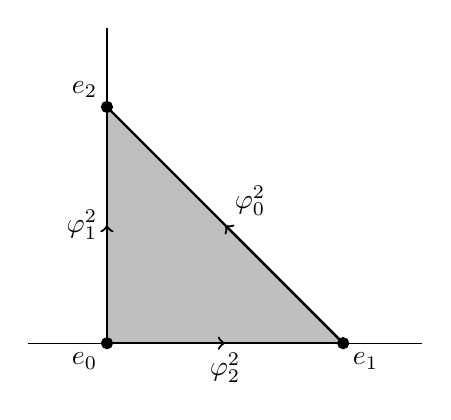
\begin{tikzpicture}[scale = 4]
    		% Draw axes
			\draw (-.25,1) -- (1,1);
			\draw (0,1) -- (0,2);
			\fill[fill=gray!50] (0,1)--(.75,1)--(0,1.75);
			\draw [thick,->] (0,1) -- (.375,1);
			\draw [thick,->] (0,1) -- (0,1.375);
			\draw [thick,->] (.75,1) -- (.375,1.375);
			\draw [thick] (0,1) -- (.75,1);
			\draw [thick] (0,1) -- (0,1.75);
			\draw [thick] (.75,1) -- (0,1.75);
			\draw[fill] (0,1) circle [radius=.5pt] node[below left]{$e_0$};
			\draw[fill] (.75,1) circle [radius=.5pt] node[below right]{$e_1$};
			\draw[fill] (0,1.75) circle [radius=.5pt] node[above left]{$e_2$};
			\node at (.375,1) [below] {$\varphi^2_2$};
			\node at (.375,1.375) [above right] {$\varphi^2_0$};
			\node at (0,1.375) [left] {$\varphi^2_1$};
		\end{tikzpicture}
		\caption{Face maps for $n = 2$.}
	\end{figure}
\end{example}
